\documentclass[a4paper,10pt]{article}
\usepackage[spanish]{babel}
\usepackage[latin1]{inputenc}
\usepackage{anysize} % Soporte para el comando \marginsize
\usepackage{listings}
\usepackage{formular}
\usepackage[pdftex]{graphicx}
\usepackage{setspace}
\usepackage{booktabs}



\DeclareGraphicsExtensions{.pdf,.png,.jpg}

\usepackage{color}
\definecolor{gray97}{gray}{.97}
\definecolor{gray75}{gray}{.75}
\definecolor{gray45}{gray}{.45}

\lstset{ frame=Ltb,
     framerule=0pt,
     aboveskip=0.5cm,
     framextopmargin=3pt,
     framexbottommargin=3pt,
     framexleftmargin=0.4cm,
     framesep=0pt,
     rulesep=.4pt,
     backgroundcolor=\color{gray97},
     rulesepcolor=\color{black},
     %
     stringstyle=\ttfamily,
     showstringspaces = false,
     basicstyle=\small\ttfamily,
     commentstyle=\color{gray45},
     keywordstyle=\bfseries,
     %
     numbers=left,
     numbersep=15pt,
     numberstyle=\tiny,
     numberfirstline = false,
     breaklines=true,
   }

% minimizar fragmentado de listados
\lstnewenvironment{listing}[1][]
   {\lstset{#1}\pagebreak[0]}{\pagebreak[0]}

\lstdefinestyle{consola}
   {basicstyle=\scriptsize\bf\ttfamily,
    backgroundcolor=\color{gray75},
   }

\lstdefinestyle{C}
   {language=C,
   }


\renewcommand*\lstlistingname{Listado}


\marginsize{3cm}{3cm}{2.5cm}{2.5cm}
\setlength{\parindent}{25pt}

%opening
\title{\textbf{ Wireless communications
in NS3}\\ Simulating wireless communications}
\author{Alejandro Juli\'an Ferro Bejerano}

\begin{document}


\maketitle

\begin{figure}[!h]
\centering
   
\includegraphics[width=8cm]{escudo_esi.jpg}
\end{figure}

\newpage

\tableofcontents

\newpage

\section{Objetives}

The main objective of this documents is to understand wireless communications and guide student in
its first simulation process through NS3 simulator.

\singlespacing
To do so, we will answer some fundamental questions. Let's look

\section{Changing the script}
Starting with the original example stats and responds as would the following activities.

\subsection{increment the distances used in each iteration of the simulation to: 25 50 75 100 125 145 147
150 152 155 157 160 162 165 167 170 172 175 177 180 185 190 195 200 210 220 230 240 250
300 350 400 450 500 600 750 1000}

\singlespacing
To resolve this issue we edit the \textbf{wifi-example-db.sh} file by changing the values of the variable "Distances"

\begin{lstlisting}[style=C]
-db.sh
#!/bin/sh

DISTANCES="25 50 75 100 125 145 147 150 152 155 157 160 162 165 167 170 172 175 177 180 185 190 195 200 210 220 230 240 250 300 350 400 450 500 600 750 1000"
(...)
\end{lstlisting}

\subsection{Reduce the number of iterations for each distance from five to one}

\singlespacing
Same as above case but editing the variable "Trials"

\begin{lstlisting}[style=C]
-db.sh
#!/bin/sh

DISTANCES="25 50 75 100 125 145 147 150 152 155 157 160 162 165 167 170 172 175 177 180 185 190 195 200 210 220 230 240 250 300 350 400 450 500 600 750 1000"
TRIALS="1"

(...)
\end{lstlisting}


\subsection{Adjust the x-axis of the gnuplot script to show results of the new distance}

\singlespacing
To adjust the x-axis of the gnuplot we only need edit the \textbf{wifi-example.gnuplot} as we show and change the value of the \emph{xrange}

\begin{lstlisting}[style=C]
(...)
#--------- x-axis adjust --------------
set xrange [0:1500]
#--------------------------------------
(...)
\end{lstlisting}


\begin{figure}[h]
        	\centering
    \includegraphics[scale=0.60]{wifi-default.eps}
    \caption{Graphic generated by example stats of NS3 with previous amendments}
    \label{fig:inicio}
        \end{figure}


\section{Changing the antenna parameters of simulation}

\subsection{which object represents the antenna? Which properties do you should change for increase the range
of a successful communication?}

\singlespacing
The object representing the antenna is \textbf{wifiPhy} and we should change the profits of reception and transmission.

\subsection{To study the values of the properties to change in order to establish a successfully communication
of 400 meters}

\singlespacing
As discussed in the previous question for successful communication, we need to edit the file \textbf{wifi-example-sim.cc}. This left in the following way.

\begin{lstlisting}[style=C]
(...)
  //--------------------------------------------
  //-- Create nodes and network stacks
  //--------------------------------------------
  NS_LOG_INFO ("Creating nodes.");
  NodeContainer nodes;
  nodes.Create (2);

  NS_LOG_INFO ("Installing WiFi and Internet stack.");
  WifiHelper wifi = WifiHelper::Default ();
  NqosWifiMacHelper wifiMac = NqosWifiMacHelper::Default ();
  wifiMac.SetType ("ns3::AdhocWifiMac");
  YansWifiPhyHelper wifiPhy = YansWifiPhyHelper::Default ();
  #--- profits of transmission and reception ---
  wifiPhy.Set("RxGain",DoubleValue(10));
  wifiPhy.Set("TxGain",DoubleValue(10));
  #---------------------------------------------
  YansWifiChannelHelper wifiChannel = YansWifiChannelHelper::Default ();
  wifiPhy.SetChannel (wifiChannel.Create ());
  NetDeviceContainer nodeDevices = wifi.Install (wifiPhy, wifiMac, nodes);

(...)
\end{lstlisting}


\begin{figure}[h]
        	\centering
    \includegraphics[scale=0.55]{wifi-400.eps}
    \caption{Graphic generated by example stats of NS3 with previous amendments}
    \label{fig:inicio}
        \end{figure}


\section{The loss model}

\subsection{Surf in the NS3 help and list the different types of loss propagation models implemented}

\singlespacing
\textbf{PropagationLossModels:}

\begin{itemize}
  \item FriisPropagationLossModel
  \item TwoRayGroundPropagationLossModel
  \item LogDistancePropagationLossModel
  \item ThreeLogDistancePropagationLossModel
  \item JakesPropagationLossModel
  \item PropagationLossModel
  \item RandomPropagationLossModel
  \item NakagamiPropagationLossModel
  \item FixedRssLossModel
  \item MatrixPropagationLossModel
  \item RangePropagationLossModel
  \item OkumuraHataPropagationLossModel
  \item ItuR1411LosPropagationLossModel
  \item ItuR1411NlosOverRooftopPropagationLossModel
  \item Kun2600MhzPropagationLossModel

\end{itemize}

\subsection{Test one of the radio propagation models using our example (check AddPropagationLoss method of
class YansWifiChannelHelper) and provide a graphic comparing the results of the YansWifiChannel
with default loss propagation model and the radio propagation model chosen by you}

\singlespacing
Disable the antenna modification done in the last section in order to have defaults settings for the
configurated loss model. In the same way increase the number of test in the area where rate of packet lost
stats to increase (for example testing every 10 meters between 100 and 200 meters if you observe that
between these two distances the loss of packets start to be different of 0).

\begin{figure}[h]
        	\centering
    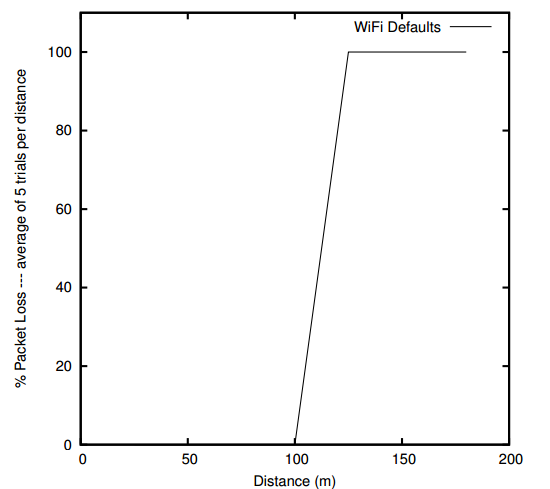
\includegraphics[scale=0.55]{basegraph.png}
    \caption{Graphic generated by example stats of NS3}
    \label{fig:inicio}
        \end{figure}


\pagebreak

\section{Webgraf\'ia y herramientas}
\begin{itemize}
\item https://www.nsnam.org/doxygen/
\item \LaTeX
\end{itemize}



\end{document}
